% ==============================================================================
% PHẦN 1: TRANG BÌA CHUẨN ĐỒ ÁN / BÀI TẬP LỚN UTH
% (Thiết kế bám sát 100% mẫu ảnh Trang bìa mẫu.png)
% ==============================================================================

\begin{titlepage}
\thispagestyle{empty}

% Dùng nguyên ảnh khung trong suốt, căn theo vùng khung bìa hiện tại.
\begin{tikzpicture}[remember picture, overlay]
  \node[inner sep=0pt] at ($(current page.center)+(5mm,0)$)
    {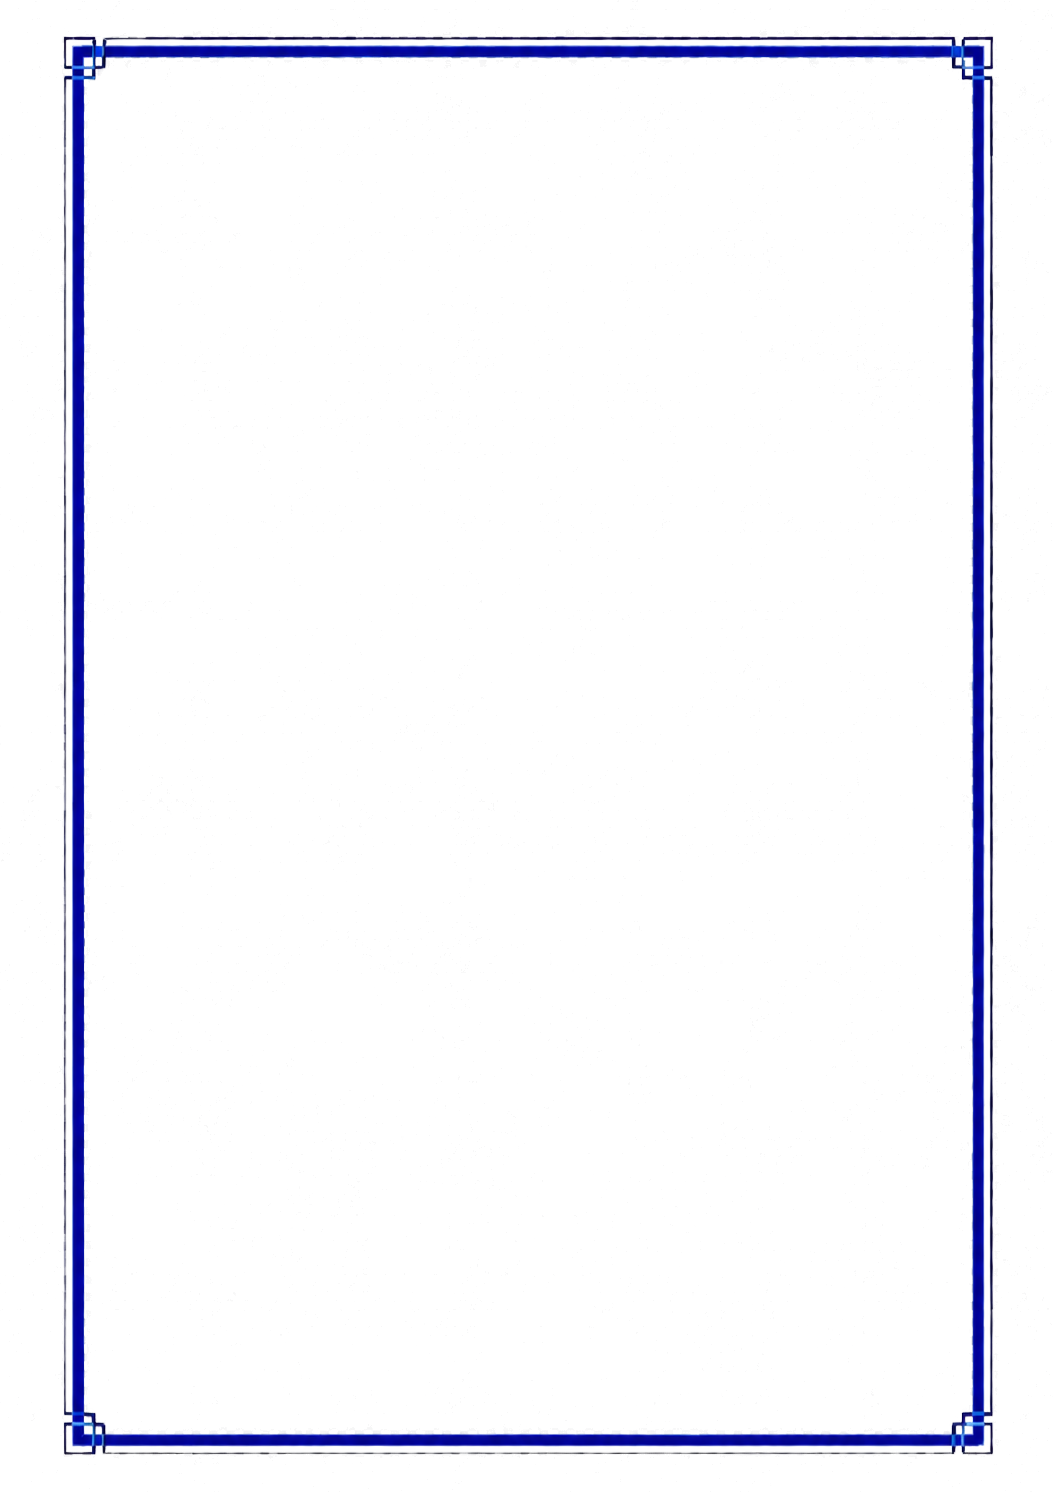
\includegraphics[width=194mm,height=275mm]{frame_transparent.png}};
\end{tikzpicture}

\vspace*{-0.6cm}

\begin{center}
  % Tiêu đề Trường
  {\fontsize{13pt}{16pt}\selectfont \textbf{\TenTruong}}\\[0.4em]
  {\fontsize{13pt}{16pt}\selectfont \textbf{VIỆN \underline{CÔNG NGHỆ THÔNG TIN VÀ ĐIỆN, ĐIỆN TỬ}}}\\[1.2cm]

  % Logo UTH
  
\includegraphics[width=6.5cm]{figures/uth_logo.png}\\[1.4cm]

  % Loại báo cáo & Môn học
  {\fontsize{14pt}{18pt}\selectfont \textbf{\LoaiBaoCao}}\\[0.5em]
  {\fontsize{14pt}{18pt}\selectfont \textbf{\TenMonHoc}}\\[1.4cm]

  % Tên Đề tài (In hoa, Đậm, Màu Đỏ theo chuẩn ảnh mẫu)
  \begin{minipage}{\textwidth}
    \centering
    {\fontsize{14pt}{20pt}\selectfont \textcolor{UTHRed}{\textbf{\TenDeTai}}}
  \end{minipage}

  \vfill

  % Khối thông tin Giảng viên hướng dẫn & Sinh viên thực hiện
  % (Căn lề phải theo đúng bố cục ảnh mẫu)
  \begin{flushright}
    \begin{minipage}{0.58\textwidth}
      \setstretch{1.2}
      {\fontsize{12pt}{15pt}\selectfont
        \textbf{GVHD:} \GiangVienHuongDan\\[0.6em]
        \textbf{SVTH:} \TenNhom\\[0.4em]
        \begin{tabular}{@{}ll@{}}
          \ThanhVienMot\\
          \ThanhVienHai\\
          \ThanhVienBa\\
          \ThanhVienBon\\
          \ThanhVienNam\\
          \ThanhVienSau\\
          \ThanhVienBay\\
        \end{tabular}
      }
    \end{minipage}
  \end{flushright}

  \vspace*{1.0cm}

  % Địa điểm và thời gian (Căn giữa cuối trang)
  {\fontsize{12pt}{14pt}\selectfont \DiaDiemThoiGian}\\[0.2cm]
\end{center}

\end{titlepage}
